\subsection{Experiments and Results}\label{sec:experiments}

Is an offline RL algorithm able to learn navigation policies effectively?
To answer this question, we have trained our DD-IQL model using the expert demonstrations on five different experimental setups.
These setups have been designed with an incremental difficulty.
The first three are evaluated on the same environments in which the agents were trained, while the last two are evaluated on different environments.
The details of the setups are depicted on figure~\ref{fig:setups}.

We compare our results with the current state-of-the-art model PirlNav~\cite{ramrakhya2023}.
This model is based on a two-phase training schedule.
The first phase is a supervised learning phase, where the model is trained using behavior cloning on the expert demonstrations.
The second phase is a reinforcement learning phase, where the model is fine-tuned using DD-PPO~algorithm~\cite{wijmans2020}.
For a fair comparison, we train the PirlNav agent using only the behavior cloning phase on the same setups as our OffNav model.

Results are shown on table~\ref{tab:success}.
It can be seen that both methods obtain similar performance on setups 1 to 3.
Offnav method outperforms PirlNav on setup 2, while PirlNav outperforms OffNav on setup 3, and both of them obtain $100\%$ SR on setup 1.
When evaluated on setup 4, PirlNav outperforms OffNav by $2.27\%$ absolute points.
However, on setup 5, the most challenging one, OffNav outperforms PirlNav by $8.69\%$ absolute points.


\begin{table}
    \centering
    \begin{tabular}{c|ccc}
        \toprule
        \textit{Experimental Setup} & \textit{OffNav}  & \textit{PirlNav} \\
        \midrule
        \textsc{Setup 1}            & 100\%          & 100\%   \\
        \textsc{Setup 2}            & \textbf{79.31\%} & 72.50\%          \\
        \textsc{Setup 3}            & 75.78\%          & \textbf{77.63\%} \\
        \textsc{Setup 4}            & 25.00\%          & \textbf{27.27\%} \\
        \textsc{Setup 5}            & \textbf{34.78\%} & 26.09\%          \\
        \bottomrule
    \end{tabular}
    \caption{Success Rate for OffNav and PirlNav methods on the five experimental setups.}
    \label{tab:success}
\end{table}

\begin{figure}
    \centering
    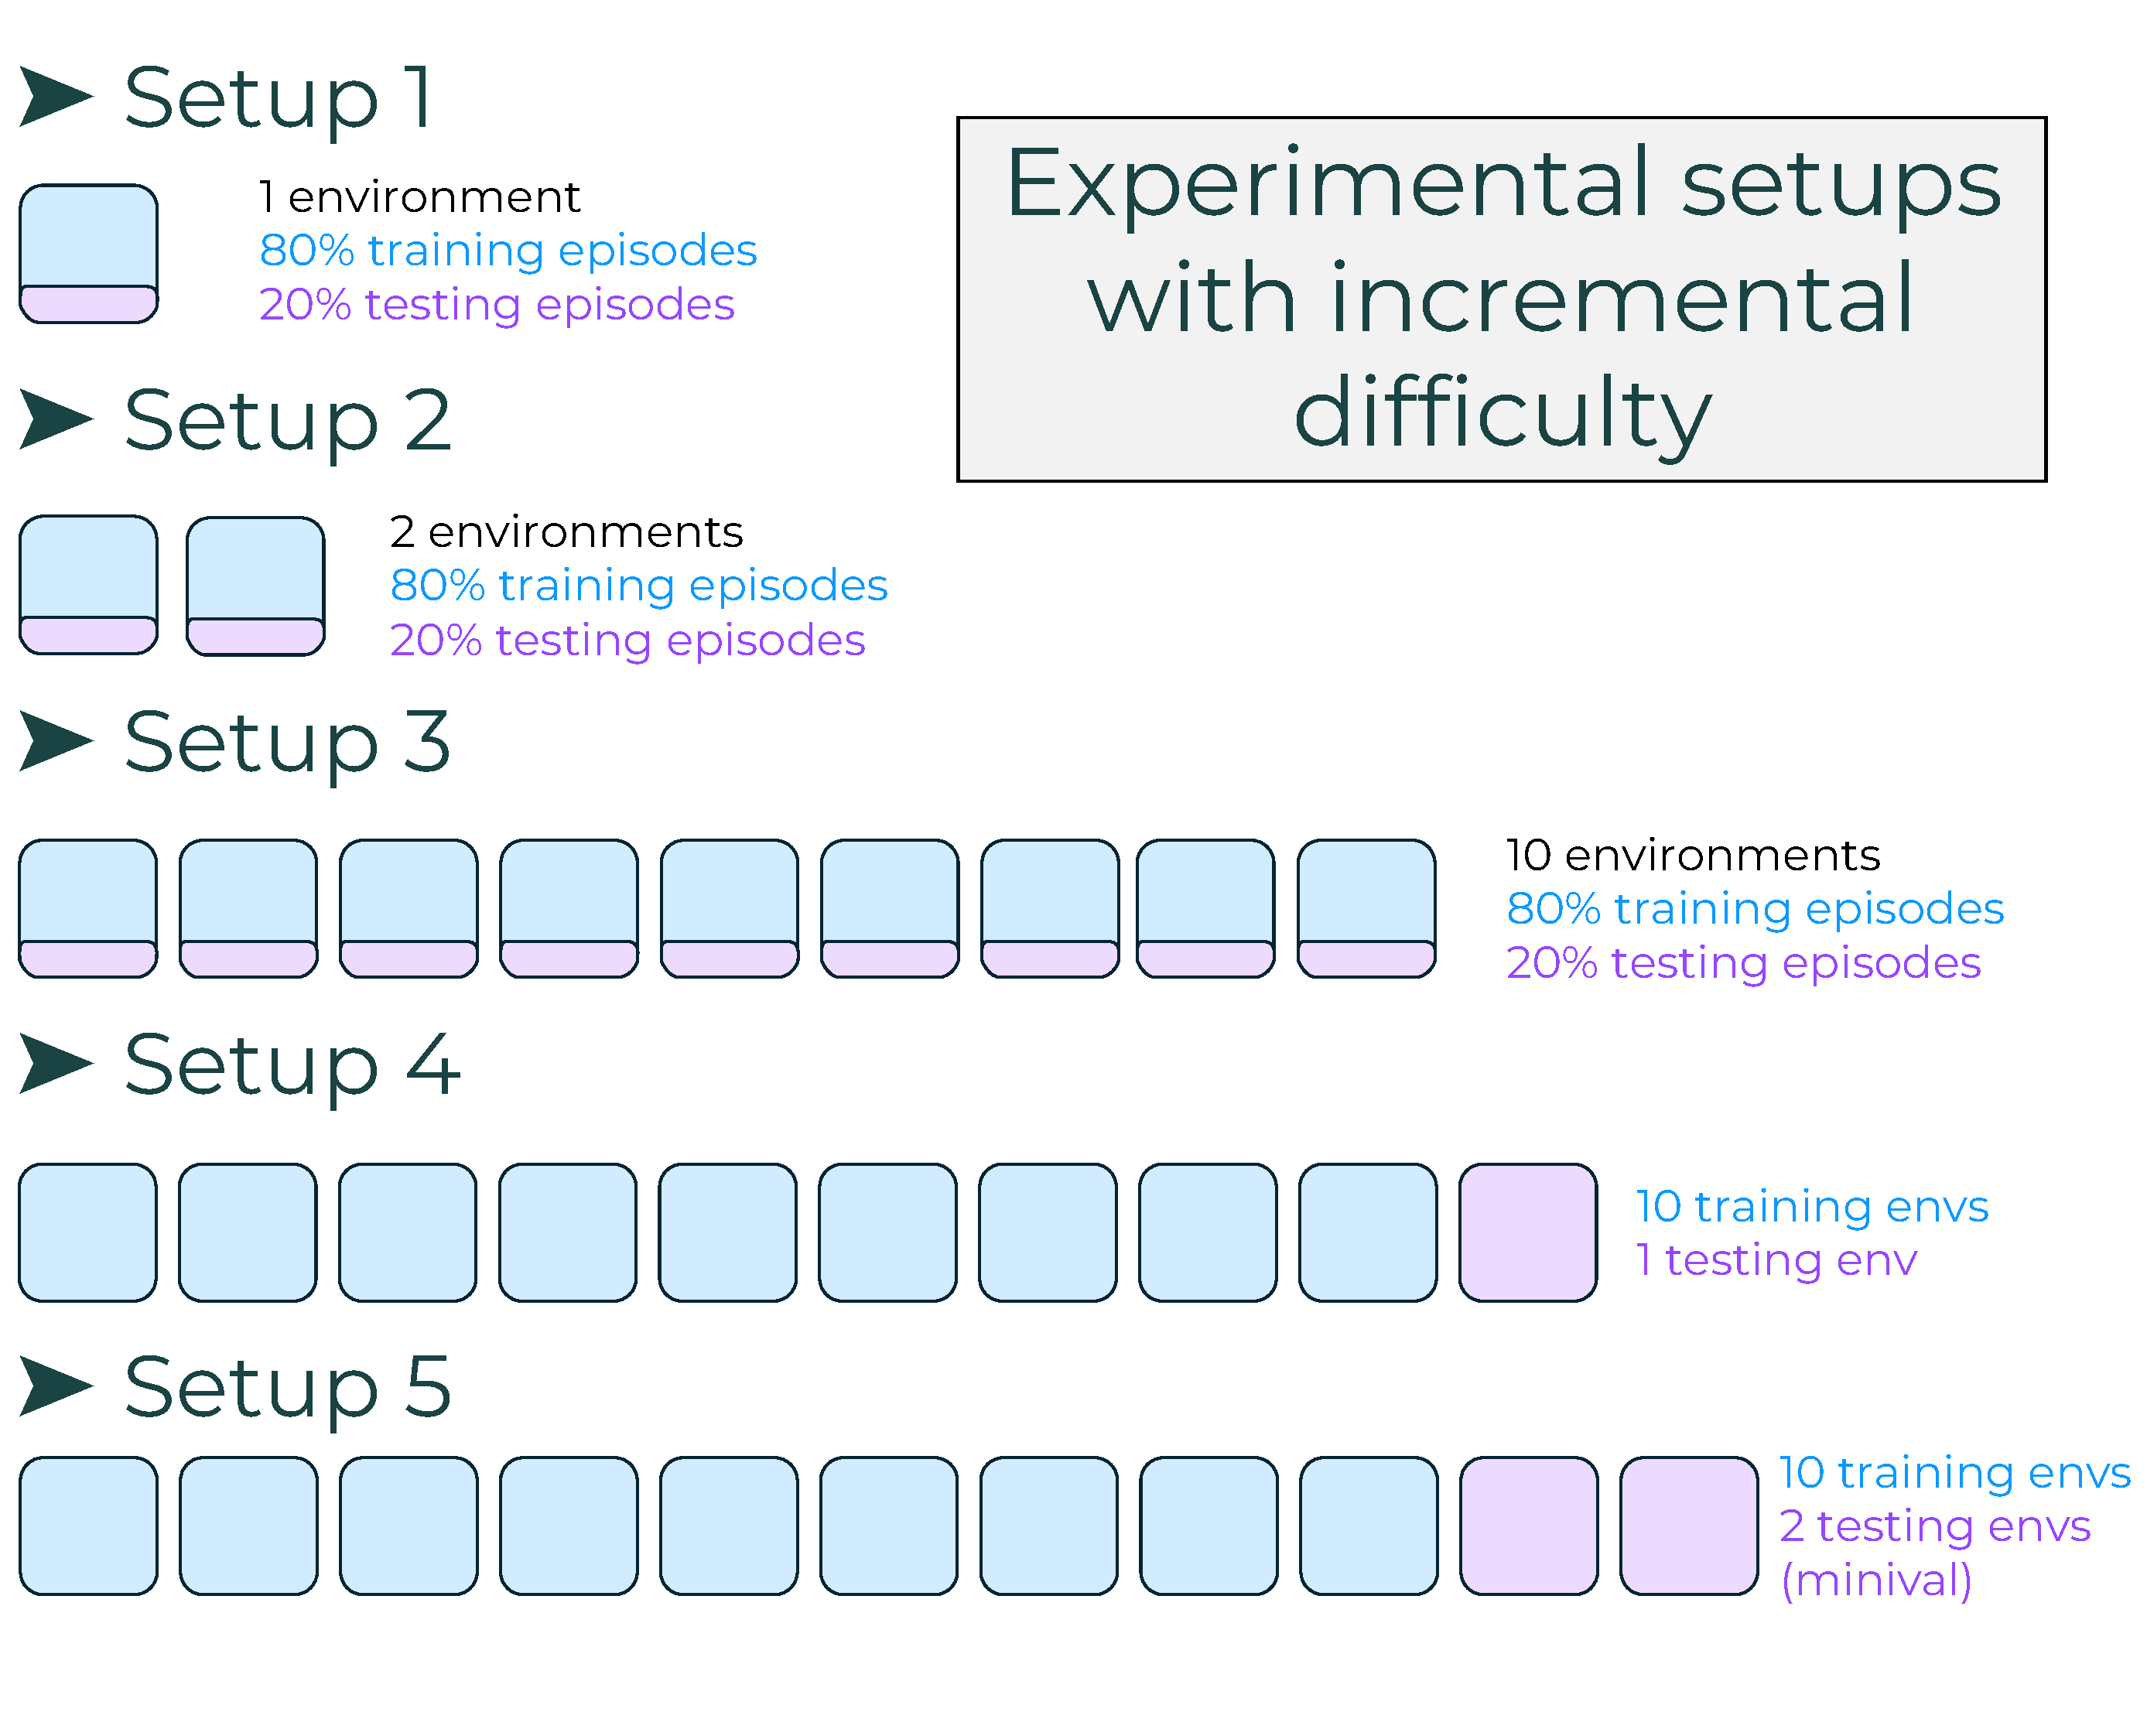
\includegraphics[width=\linewidth]{figures/offnav/experimental_setups}
    \caption{Five experimental setups designed with an incremental difficulty.}
    \label{fig:setups}
\end{figure}




